%===============================================================================
% LaTeX sjabloon voor de bachelorproef toegepaste informatica aan HOGENT
% Meer info op https://github.com/HoGentTIN/latex-hogent-report
%===============================================================================

\documentclass[dutch,dit,thesis]{hogentreport}

% TODO:
% - If necessary, replace the option `dit`' with your own department!
%   Valid entries are dbo, dbt, dgz, dit, dlo, dog, dsa, soa
% - If you write your thesis in English (remark: only possible after getting
%   explicit approval!), remove the option "dutch," or replace with "english".

\usepackage{lipsum} % For blind text, can be removed after adding actual content

%% Pictures to include in the text can be put in the graphics/ folder
\graphicspath{{../graphics/}}

%% For source code highlighting, requires pygments to be installed
%% Compile with the -shell-escape flag!
%% \usepackage[chapter]{minted}
%% If you compile with the make_thesis.{bat,sh} script, use the following
%% import instead:
\usepackage[chapter,outputdir=../output]{minted}
\usemintedstyle{solarized-light}

%% Formatting for minted environments.
\setminted{%
    autogobble,
    frame=lines,
    breaklines,
    linenos,
    tabsize=4
}

%% Ensure the list of listings is in the table of contents
\renewcommand\listoflistingscaption{%
    \IfLanguageName{dutch}{Lijst van codefragmenten}{List of listings}
}
\renewcommand\listingscaption{%
    \IfLanguageName{dutch}{Codefragment}{Listing}
}
\renewcommand*\listoflistings{%
    \cleardoublepage\phantomsection\addcontentsline{toc}{chapter}{\listoflistingscaption}%
    \listof{listing}{\listoflistingscaption}%
}

% Other packages not already included can be imported here

%%---------- Document metadata -------------------------------------------------
% TODO: Replace this with your own information
\author{Ernst Aarden}
\supervisor{Dhr. F. Van Houte}
\cosupervisor{Mevr. S. Beeckman}
\title[Optionele ondertitel]%
    {Titel van de bachelorproef}
\academicyear{\advance\year by -1 \the\year--\advance\year by 1 \the\year}
\examperiod{1}
\degreesought{\IfLanguageName{dutch}{Professionele bachelor in de toegepaste informatica}{Bachelor of applied computer science}}
\partialthesis{false} %% To display 'in partial fulfilment'
%\institution{Internshipcompany BVBA.}

%% Add global exceptions to the hyphenation here
\hyphenation{back-slash}

%% The bibliography (style and settings are  found in hogentthesis.cls)
\addbibresource{bachproef.bib}            %% Bibliography file
\addbibresource{../voorstel/voorstel.bib} %% Bibliography research proposal
\defbibheading{bibempty}{}

%% Prevent empty pages for right-handed chapter starts in twoside mode
\renewcommand{\cleardoublepage}{\clearpage}

\renewcommand{\arraystretch}{1.2}

%% Content starts here.
\begin{document}

%---------- Front matter -------------------------------------------------------

\frontmatter

\hypersetup{pageanchor=false} %% Disable page numbering references
%% Render a Dutch outer title page if the main language is English
\IfLanguageName{english}{%
    %% If necessary, information can be changed here
    \degreesought{Professionele Bachelor toegepaste informatica}%
    \begin{otherlanguage}{dutch}%
       \maketitle%
    \end{otherlanguage}%
}{}

%% Generates title page content
\maketitle
\hypersetup{pageanchor=true}

%%=============================================================================
%% Voorwoord
%%=============================================================================

\chapter*{\IfLanguageName{dutch}{Woord vooraf}{Preface}}%
\label{ch:voorwoord}

%% TODO:
%% Het voorwoord is het enige deel van de bachelorproef waar je vanuit je
%% eigen standpunt (``ik-vorm'') mag schrijven. Je kan hier bv. motiveren
%% waarom jij het onderwerp wil bespreken.
%% Vergeet ook niet te bedanken wie je geholpen/gesteund/... heeft

\lipsum[1-2]
%%=============================================================================
%% Samenvatting
%%=============================================================================

% TODO: De "abstract" of samenvatting is een kernachtige (~ 1 blz. voor een
% thesis) synthese van het document.
%
% Een goede abstract biedt een kernachtig antwoord op volgende vragen:
%
% 1. Waarover gaat de bachelorproef?
% 2. Waarom heb je er over geschreven?
% 3. Hoe heb je het onderzoek uitgevoerd?
% 4. Wat waren de resultaten? Wat blijkt uit je onderzoek?
% 5. Wat betekenen je resultaten? Wat is de relevantie voor het werkveld?
%
% Daarom bestaat een abstract uit volgende componenten:
%
% - inleiding + kaderen thema
% - probleemstelling
% - (centrale) onderzoeksvraag
% - onderzoeksdoelstelling
% - methodologie
% - resultaten (beperk tot de belangrijkste, relevant voor de onderzoeksvraag)
% - conclusies, aanbevelingen, beperkingen
%
% LET OP! Een samenvatting is GEEN voorwoord!

%%---------- Nederlandse samenvatting -----------------------------------------
%
% TODO: Als je je bachelorproef in het Engels schrijft, moet je eerst een
% Nederlandse samenvatting invoegen. Haal daarvoor onderstaande code uit
% commentaar.
% Wie zijn bachelorproef in het Nederlands schrijft, kan dit negeren, de inhoud
% wordt niet in het document ingevoegd.

\IfLanguageName{english}{%
\selectlanguage{dutch}
\chapter*{Samenvatting}
\lipsum[1-4]
\selectlanguage{english}
}{}

%%---------- Samenvatting -----------------------------------------------------
% De samenvatting in de hoofdtaal van het document

\chapter*{\IfLanguageName{dutch}{Samenvatting}{Abstract}}

\lipsum[1-4]


%---------- Inhoud, lijst figuren, ... -----------------------------------------

\tableofcontents

% In a list of figures, the complete caption will be included. To prevent this,
% ALWAYS add a short description in the caption!
%
%  \caption[short description]{elaborate description}
%
% If you do, only the short description will be used in the list of figures

\listoffigures

% If you included tables and/or source code listings, uncomment the appropriate
% lines.
\listoftables

\listoflistings

% Als je een lijst van afkortingen of termen wil toevoegen, dan hoort die
% hier thuis. Gebruik bijvoorbeeld de ``glossaries'' package.
% https://www.overleaf.com/learn/latex/Glossaries

%---------- Kern ---------------------------------------------------------------

\mainmatter{}

% De eerste hoofdstukken van een bachelorproef zijn meestal een inleiding op
% het onderwerp, literatuurstudie en verantwoording methodologie.
% Aarzel niet om een meer beschrijvende titel aan deze hoofdstukken te geven of
% om bijvoorbeeld de inleiding en/of stand van zaken over meerdere hoofdstukken
% te verspreiden!

%%=============================================================================
%% Inleiding
%%=============================================================================

\chapter{\IfLanguageName{dutch}{Inleiding}{Introduction}}%
\label{ch:inleiding}

De inleiding moet de lezer net genoeg informatie verschaffen om het onderwerp te begrijpen en in te zien waarom de onderzoeksvraag de moeite waard is om te onderzoeken. In de inleiding ga je literatuurverwijzingen beperken, zodat de tekst vlot leesbaar blijft. Je kan de inleiding verder onderverdelen in secties als dit de tekst verduidelijkt. Zaken die aan bod kunnen komen in de inleiding~\autocite{Pollefliet2011}:

\begin{itemize}
  \item context, achtergrond
  \item afbakenen van het onderwerp
  \item verantwoording van het onderwerp, methodologie
  \item probleemstelling
  \item onderzoeksdoelstelling
  \item onderzoeksvraag
  \item \ldots
\end{itemize}

\section{\IfLanguageName{dutch}{Probleemstelling}{Problem Statement}}%
\label{sec:probleemstelling}

Uit je probleemstelling moet duidelijk zijn dat je onderzoek een meerwaarde heeft voor een concrete doelgroep. De doelgroep moet goed gedefinieerd en afgelijnd zijn. Doelgroepen als ``bedrijven,'' ``KMO's'', systeembeheerders, enz.~zijn nog te vaag. Als je een lijstje kan maken van de personen/organisaties die een meerwaarde zullen vinden in deze bachelorproef (dit is eigenlijk je steekproefkader), dan is dat een indicatie dat de doelgroep goed gedefinieerd is. Dit kan een enkel bedrijf zijn of zelfs één persoon (je co-promotor/opdrachtgever).

\section{\IfLanguageName{dutch}{Onderzoeksvraag}{Research question}}%
\label{sec:onderzoeksvraag}

Wees zo concreet mogelijk bij het formuleren van je onderzoeksvraag. Een onderzoeksvraag is trouwens iets waar nog niemand op dit moment een antwoord heeft (voor zover je kan nagaan). Het opzoeken van bestaande informatie (bv. ``welke tools bestaan er voor deze toepassing?'') is dus geen onderzoeksvraag. Je kan de onderzoeksvraag verder specifiëren in deelvragen. Bv.~als je onderzoek gaat over performantiemetingen, dan 

\section{\IfLanguageName{dutch}{Onderzoeksdoelstelling}{Research objective}}%
\label{sec:onderzoeksdoelstelling}

Wat is het beoogde resultaat van je bachelorproef? Wat zijn de criteria voor succes? Beschrijf die zo concreet mogelijk. Gaat het bv.\ om een proof-of-concept, een prototype, een verslag met aanbevelingen, een vergelijkende studie, enz.

\section{\IfLanguageName{dutch}{Opzet van deze bachelorproef}{Structure of this bachelor thesis}}%
\label{sec:opzet-bachelorproef}

% Het is gebruikelijk aan het einde van de inleiding een overzicht te
% geven van de opbouw van de rest van de tekst. Deze sectie bevat al een aanzet
% die je kan aanvullen/aanpassen in functie van je eigen tekst.

De rest van deze bachelorproef is als volgt opgebouwd:

In Hoofdstuk~\ref{ch:stand-van-zaken} wordt een overzicht gegeven van de stand van zaken binnen het onderzoeksdomein, op basis van een literatuurstudie.

In Hoofdstuk~\ref{ch:methodologie} wordt de methodologie toegelicht en worden de gebruikte onderzoekstechnieken besproken om een antwoord te kunnen formuleren op de onderzoeksvragen.

% TODO: Vul hier aan voor je eigen hoofstukken, één of twee zinnen per hoofdstuk

In Hoofdstuk~\ref{ch:conclusie}, tenslotte, wordt de conclusie gegeven en een antwoord geformuleerd op de onderzoeksvragen. Daarbij wordt ook een aanzet gegeven voor toekomstig onderzoek binnen dit domein.
\chapter{\IfLanguageName{dutch}{Stand van zaken}{State of the art}}%
\label{ch:stand-van-zaken}

% Tip: Begin elk hoofdstuk met een paragraaf inleiding die beschrijft hoe
% dit hoofdstuk past binnen het geheel van de bachelorproef. Geef in het
% bijzonder aan wat de link is met het vorige en volgende hoofdstuk.

% Pas na deze inleidende paragraaf komt de eerste sectiehoofding.

Dit hoofdstuk bevat je literatuurstudie. De inhoud gaat verder op de inleiding, maar zal het onderwerp van de bachelorproef *diepgaand* uitspitten. De bedoeling is dat de lezer na lezing van dit hoofdstuk helemaal op de hoogte is van de huidige stand van zaken (state-of-the-art) in het onderzoeksdomein. Iemand die niet vertrouwd is met het onderwerp, weet nu voldoende om de rest van het verhaal te kunnen volgen, zonder dat die er nog andere informatie moet over opzoeken \autocite{Pollefliet2011}.

Je verwijst bij elke bewering die je doet, vakterm die je introduceert, enz.\ naar je bronnen. In \LaTeX{} kan dat met het commando \texttt{$\backslash${textcite\{\}}} of \texttt{$\backslash${autocite\{\}}}. Als argument van het commando geef je de ``sleutel'' van een ``record'' in een bibliografische databank in het Bib\LaTeX{}-formaat (een tekstbestand). Als je expliciet naar de auteur verwijst in de zin (narratieve referentie), gebruik je \texttt{$\backslash${}textcite\{\}}. Soms is de auteursnaam niet expliciet een onderdeel van de zin, dan gebruik je \texttt{$\backslash${}autocite\{\}} (referentie tussen haakjes). Dit gebruik je bv.~bij een citaat, of om in het bijschrift van een overgenomen afbeelding, broncode, tabel, enz. te verwijzen naar de bron. In de volgende paragraaf een voorbeeld van elk.

\textcite{Knuth1998} schreef een van de standaardwerken over sorteer- en zoekalgoritmen. Experten zijn het erover eens dat cloud computing een interessante opportuniteit vormen, zowel voor gebruikers als voor dienstverleners op vlak van informatietechnologie~\autocite{Creeger2009}.

Let er ook op: het \texttt{cite}-commando voor de punt, dus binnen de zin. Je verwijst meteen naar een bron in de eerste zin die erop gebaseerd is, dus niet pas op het einde van een paragraaf.

\begin{figure}
  \centering
  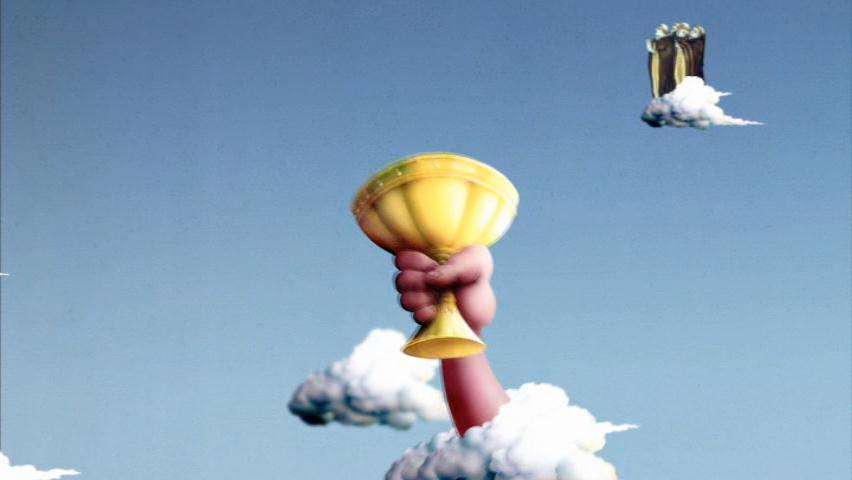
\includegraphics[width=0.8\textwidth]{grail.jpg}
  \caption[Voorbeeld figuur.]{\label{fig:grail}Voorbeeld van invoegen van een figuur. Zorg altijd voor een uitgebreid bijschrift dat de figuur volledig beschrijft zonder in de tekst te moeten gaan zoeken. Vergeet ook je bronvermelding niet!}
\end{figure}

\begin{listing}
  \begin{minted}{python}
    import pandas as pd
    import seaborn as sns

    penguins = sns.load_dataset('penguins')
    sns.relplot(data=penguins, x="flipper_length_mm", y="bill_length_mm", hue="species")
  \end{minted}
  \caption[Voorbeeld codefragment]{Voorbeeld van het invoegen van een codefragment.}
\end{listing}

\lipsum[7-20]

\begin{table}
  \centering
  \begin{tabular}{lcr}
    \toprule
    \textbf{Kolom 1} & \textbf{Kolom 2} & \textbf{Kolom 3} \\
    $\alpha$         & $\beta$          & $\gamma$         \\
    \midrule
    A                & 10.230           & a                \\
    B                & 45.678           & b                \\
    C                & 99.987           & c                \\
    \bottomrule
  \end{tabular}
  \caption[Voorbeeld tabel]{\label{tab:example}Voorbeeld van een tabel.}
\end{table}


%%=============================================================================
%% Methodologie
%%=============================================================================

\chapter{\IfLanguageName{dutch}{Methodologie}{Methodology}}%
\label{ch:methodologie}

%% TODO: In dit hoofstuk geef je een korte toelichting over hoe je te werk bent
%% gegaan. Verdeel je onderzoek in grote fasen, en licht in elke fase toe wat
%% de doelstelling was, welke deliverables daar uit gekomen zijn, en welke
%% onderzoeksmethoden je daarbij toegepast hebt. Verantwoord waarom je
%% op deze manier te werk gegaan bent.
%% 
%% Voorbeelden van zulke fasen zijn: literatuurstudie, opstellen van een
%% requirements-analyse, opstellen long-list (bij vergelijkende studie),
%% selectie van geschikte tools (bij vergelijkende studie, "short-list"),
%% opzetten testopstelling/PoC, uitvoeren testen en verzamelen
%% van resultaten, analyse van resultaten, ...
%%
%% !!!!! LET OP !!!!!
%%
%% Het is uitdrukkelijk NIET de bedoeling dat je het grootste deel van de corpus
%% van je bachelorproef in dit hoofstuk verwerkt! Dit hoofdstuk is eerder een
%% kort overzicht van je plan van aanpak.
%%
%% Maak voor elke fase (behalve het literatuuronderzoek) een NIEUW HOOFDSTUK aan
%% en geef het een gepaste titel.

\lipsum[21-25]



% Voeg hier je eigen hoofdstukken toe die de ``corpus'' van je bachelorproef
% vormen. De structuur en titels hangen af van je eigen onderzoek. Je kan bv.
% elke fase in je onderzoek in een apart hoofdstuk bespreken.

%\input{...}
%\input{...}
%...

%%=============================================================================
%% Conclusie
%%=============================================================================

\chapter{Conclusie}%
\label{ch:conclusie}

% TODO: Trek een duidelijke conclusie, in de vorm van een antwoord op de
% onderzoeksvra(a)g(en). Wat was jouw bijdrage aan het onderzoeksdomein en
% hoe biedt dit meerwaarde aan het vakgebied/doelgroep? 
% Reflecteer kritisch over het resultaat. In Engelse teksten wordt deze sectie
% ``Discussion'' genoemd. Had je deze uitkomst verwacht? Zijn er zaken die nog
% niet duidelijk zijn?
% Heeft het onderzoek geleid tot nieuwe vragen die uitnodigen tot verder 
%onderzoek?

\lipsum[76-80]



%---------- Bijlagen -----------------------------------------------------------

\appendix

\chapter{Onderzoeksvoorstel}

Het onderwerp van deze bachelorproef is gebaseerd op een onderzoeksvoorstel dat vooraf werd beoordeeld door de promotor. Dat voorstel is opgenomen in deze bijlage.

%% TODO: 
%\section*{Samenvatting}

% Kopieer en plak hier de samenvatting (abstract) van je onderzoeksvoorstel.

% Verwijzing naar het bestand met de inhoud van het onderzoeksvoorstel
%---------- Inleiding ---------------------------------------------------------

% TODO: Is dit voorstel gebaseerd op een paper van Research Methods die je
% vorig jaar hebt ingediend? Heb je daarbij eventueel samengewerkt met een
% andere student?
% Zo ja, haal dan de tekst hieronder uit commentaar en pas aan.

%\paragraph{Opmerking}

% Dit voorstel is gebaseerd op het onderzoeksvoorstel dat werd geschreven in het
% kader van het vak Research Methods dat ik (vorig/dit) academiejaar heb
% uitgewerkt (met medesturent VOORNAAM NAAM als mede-auteur).
% 

\section{Inleiding}%
\label{sec:inleiding}
Deze bachelorproef richt zich op een specifiek probleem binnen DEME-Group, een internationaal bedrijf dat zich specialiseert in maritieme projecten, waaronder 
baggerwerkzaamheden, \\offshore-activiteiten en infrastructuurwerken. \\DEME-Group heeft meer dan 100 schepen die wereldwijd worden ingezet voor verschillende maritieme projecten. Het probleem 
bevindt zich echter binnen de netwerkstructuur op hun schepen. Deze bachelorproef zoomt in op de netwerkstructuur en nurse-PC op één bepaald schip. De netwerkstructuur bestaat uit twee netwerken: het IT-netwerk voor administratieve taken 
en het OT-netwerk voor de operationele systemen. Deze twee netwerken zijn met elkaar verbonden via de nurse-PC, 
die fungeert als schakel en toegangspunt tussen deze twee netwerken. De focus van deze bachelorproef ligt op het afbakenen en versterken van die schakel.

\subsection{Probleemstelling en hoofdonderzoeksvraag}
De ingenieurs van het ELEK-team aan boord moeten snel en efficiënt problemen via de nurse-PC oplossen wanneer zich storingen voordoen in het OT- of  IT-netwerk.  
Als het probleem niet snel wordt opgelost, kunnen belangrijke werkzaamheden, zoals bijvoorbeeld het vertrek van het schip of het baggerwerkzaambheden, niet doorgaan. 
Dit brengt aanzienlijke kosten met zich mee. De nurse-PC wordt echter vaak misbruikt voor niet-geautoriseerde activiteiten. Dit heet Shadow IT en leidt tot verlies van controle 
over de beveiliging en toegang tot de nurse-PC. Hierdoor nemen de risico’s voor beide netwerken aan boord toe. Het is daarom van cruciaal belang om de nurse-PC af 
te bakenen: het toegangsbeheer te optimaliseren en de beveiliging te versterken. Op basis van deze probleemstelling volgt de hoofdonderzoeksvraag: 
"Hoe kan het toegangsbeheer van de nurse-PC op een schip worden versterkt om de veiligheid van zowel het IT- als OT-netwerk aan boord te garanderen?” 

\subsection{Deelvragen}
- Hoe is het IT- en OT-netwerk ingericht in relatie tot de nurse-PC aan boord van een schip? \\     
- Op welke wijze wordt toegang verleend tot de nurse-PC zowel intern als extern? \\    
- Wat zijn de specifieke kwetsbaarheden van de nurse-PC op basis van het toegangsbeheer? \\       
- Welke beveiligingsmaatregelen moeten worden geïmplementeerd op basis van de bevindingen uit de vulnerability assessment van het toegangsbeheer? \\
- Welke methoden kunnen worden gebruikt om Shadow IT beter te detecteren en in kaart te brengen? \\
- Hoe kan Shadow IT bijdragen aan de verspreiding van malware of andere cyberdreigingen binnen het netwerk?\\
- Wat zijn de gevolgen van Shadow IT met betrekking tot de regelgeving aan boord?\\
- Op welke manier kunnen ongeautoriseerde gebruikers toegang krijgen tot de nurse-PC?\\

\subsection{Doelgroep}
Een goed functionerende nurse-PC en veilige netwerken zijn essentieel voor de continuïteit van alle operaties aan boord. 
Dit kan de primaire doelgroep DEME-Group, helpen om de netwerkbeveiliging te verbeteren en financiële verliezen door storingen te voorkomen.
Binnen het bedrijf worden drie specifieke groepen als doelgroepen beschouwd: het ELEK-team aan boord, de systeem- en netwerkbeheerders voor zowel het IT- als het OT-netwerk, de scheepsoperators en de leidinggevenden.
Het ELEK-team, bestaande uit verschillende ingenieurs met elk hun eigen specialisatie, is verantwoordelijk voor het onderhoud en de werking van de operationele systemen aan boord. Bij technische problemen dienen zij snel en efficiënt te troubleshooten met de nurse-PC.  
Een veilige en goed afgebakende nurse-PC is voor hen van cruciaal belang om zonder vertraging toegang te krijgen tot de juiste systemen, om storingen in de IT- en OT-netwerken snel te verhelpen zodat het schip operationeel blijft.
De systeem -en netwerkbeheerders moeten ervoor zorgen dat onbevoegden geen toegang krijgen en dat de systemen beschermd zijn tegen cyberbedreigingen. Dit zal bijdragen aan de algemene netwerkbeveiliging.
Scheepsoperators en hun leidinggevenden (o.a. de kapitein, eerste stuurman, enz.) zijn verantwoordelijk voor de operationele veiligheid en efficiëntie aan boord. Een veilige nurse-PC is voor hen van groot belang om storingen te voorkomen, 
zodat de schepen probleemloos kunnen opereren en de veiligheid van de bemanning gewaarborgd blijft.

\subsection{Onderzoeksdoelstelling}
De onderzoeksdoelstelling is het opstellen van een gedetailleerd rapport waarin de geïdentificeerde kwetsbaarheden en aanbevelingen, als resultaat van de vulnerability assesment, worden genoteerd.
Op basis van dit rapport wordt er een proof-of-concept gedemonstreerd met alle beveiligingsimplementaties.
Daarnaast wordt er ook documentatie bijgehouden van alle stappen van de technische implementatie.
Het doel van de documentatie is dat de basis van de proof-of-concept in de toekomst kan worden gerepliceerd en herbruikt op de gehele vloot van DEME-Group.


%---------- Stand van zaken ---------------------------------------------------

\section{Literatuurstudie}%
\label{sec:literatuurstudie}
\subsection{Introductie}
In de afgelopen jaren is de kwetsbaarheid van schepen voor cyberaanvallen in een verontrustend tempo toegenomen. Weston \textcite{Hecker2021}, ethical hacker bij het security bedrijf 
Mission Secure, benadrukt in een interview met Declan Bush de vaak over het hoofd geziene zwaktes in de maritieme beveiliging. Hij
legt uit hoe kwetsbaar veel schepen zijn, ondanks de vooruitgang in informatiebeveiliging. \textcite{Hecker2021} bevestigt hoe schijnbaar onschuldige apparaten, zoals draadloze toetsenborden, printers en 
zelfs gebruikershandleidingen, door aanvallers kunnen worden misbruikt. Dit illustreert de gevaren van shadow IT, waarbij bijvoorbeeld 
ongecontroleerde en niet-geautoriseerde apparaten aan de nurse-PC kunnen worden gekoppeld, wat een groot risico vormt voor de operationele technologie aan boord. 
Deze technologie is vaak het belangrijkste doelwit voor aanvallers omdat deze systemen verantwoordelijk zijn voor de werking van het schip.

\subsection{De rol van de nurse-PC}
De Nurse-PC speelt de belangrijkste rol in de brugfunctie tussen het IT- en OT-netwerk. Deze specifieke computer bevindt 
zich tussen beide netwerken en fungeert als toegangspunt en tussenpersoon die belangrijke informatie en documentatie kan ophalen over verschillende systemen.
Het systeem stelt de technici in staat om toegang te krijgen tot gedetailleerde gegevens over de 
machines, zodat ze snel kunnen troubleshooten en technische problemen kunnen oplossen. De Nurse-PC zorgt ervoor dat alle benodigde documentatie
snel beschikbaar is voor het onderhoudsteam. Zo kunnen zij de juiste acties ondernemen om storingen 
te verhelpen en de systemen optimaal te laten functioneren (K. Ternoey, persoonlijke communicatie, 4 november 2024).

\subsection{Wat is Shadow IT}
Naast cyberaanvallen kunnen er ook schadelijke situaties ontstaan door Shadow IT binnen de organisatie. Hoewel dit vaak onbedoeld gebeurt, vormt dit probleem een 
grotere bedreiging dan externe aanvallen. Shadow IT verwijst naar IT-middelen die binnen een organisatie worden gebruikt zonder goedkeuring of beheer door de IT-afdeling. 
Dit kan variëren van persoonlijke apparaten tot cloudtechnologieën. Dergelijke technologieën zijn vaak niet in overeenstemming met de interne IT-processen en beveiligingsmaatregelen, waardoor ze een 
risico vormen voor de veiligheid van gegevens en systemen. Shadow IT kan leiden tot datadiefstal, 
verspreiding van malware of andere beveiligingsincidenten, omdat deze apparaten of diensten vaak niet voldoen aan de vereiste beveiligingsnormen. Hoewel het meestal niet opzettelijk is, 
ontstaat Shadow IT vaak doordat medewerkers officiële tools of processen als onvoldoende beschouwen om hun werk effectief te kunnen uitvoeren. Het is van essentieel belang dat organisaties 
deze praktijken herkennen en beheren om de bijbehorende risico’s te beperken \autocite{NCSC2023}.

\subsection{Shadow IT in de context van de Nurse-PC}
In de context van de nurse-PC aan boord van een schip vormt Shadow IT een ernstig probleem. Wanneer medewerkers persoonlijke apparaten of 
niet-goedgekeurde software gebruiken om toegang te krijgen tot systemen of gegevens, kunnen er ernstige beveiligingsproblemen ontstaan. 
Bijvoorbeeld, als de nurse-PC wordt gekoppeld aan onveilige hardware of software, kunnen gevoelige gegevens kwetsbaar worden voor datadiefstal of aanvallen, zoals eerder besproken in het interview met \textcite{Hecker2021}. 
Bovendien kunnen werknemers die betrokken zijn bij Shadow IT malware binnenhalen via niet-geautoriseerde apparaten of software, die zich via de nurse-PC kunnen verspreiden naar zowel 
het IT- als het OT-netwerk. Dit vergroot de kans op systeeminfecties, waardoor de integriteit van de machinebesturingssystemen ernstig in gevaar kan komen. (K. Ternoey, persoonlijke communicatie, 4 november 2024).

\subsection{Het verschil tussen een IT-netwerk en een OT-netwerk}
IT (informatietechnologie) en OT (operationele technologie) vervullen verschillende functies binnen een organisatie. IT richt zich op de verwerking, opslag en 
uitwisseling van gegevens, waarbij computers, servers en andere apparaten zoals smartphones en tablets worden gebruikt. OT daarentegen houdt zich bezig met het 
monitoren en besturen van fysieke processen en apparatuur, zoals industriële machines en besturingssystemen. Hoewel deze twee netwerken lange tijd gescheiden waren, 
wordt de scheidslijn steeds vager door de opkomst van IT/OT-convergentie, waarbij beide systemen steeds meer met elkaar worden geïntegreerd. Dit biedt nieuwe kansen, 
maar brengt ook risico’s met zich mee, vooral op het gebied van cybersecurity \autocite{onlogic2023}.

\subsection{IT/OT-convergentie}
De convergentie van Informatie Technologie (IT) en Operationele Technologie (OT) is een proces waarbij de twee voorheen gescheiden werelden worden geïntegreerd, mede aangedreven door digitale 
transformatie en technologische innovaties zoals Internet of Things (IoT) en big data-analyse. Deze integratie maakt een naadloze gegevensstroom mogelijk tussen de digitale en fysieke werelden, 
waardoor operationele systemen efficiënter kunnen worden aangestuurd en geoptimaliseerd. Er zijn drie belangrijke vormen van IT/OT-convergentie: fysieke convergentie (directe verbinding van OT-apparaten met IT-netwerken), 
softwareconvergentie \\(waarbij OT-gegevens digitaal worden geanalyseerd door IT-systemen), en organisatorische convergentie (waarbij de werkstromen van IT en OT samensmelten om de samenwerking te verbeteren). Deze integratie 
leidt tot betere besluitvorming, verhoogde efficiëntie en innovatie, wat cruciaal is voor de vooruitgang van de Industrie 4.0 en het Industrial Internet of Things (IIoT) \autocite{maleh2021ot,paloaltonetworks2023}.

\subsection{OT-security}
OT-security richt zich op de bescherming van operationele technologieën die worden gebruikt in industriële netwerken. Naarmate de connectiviteit van deze systemen 
met externe netwerken toeneemt, nemen de risico’s van cyberaanvallen toe. OT-security omvat een breed scala aan maatregelen en technologieën die ontworpen zijn om 
de betrouwbaarheid en veiligheid van industriële systemen te waarborgen, zoals SCADA (Supervisory Control And Data Acquisition) en Industrial Control Systems (ICS). Deze systemen worden vaak ingezet in vitale 
sectoren zoals energie, transport en de scheepvaart. De integratie van IT- en OT-netwerken, bekend als IT/OT-convergentie, biedt meer efficiëntie, maar brengt ook nieuwe 
beveiligingsuitdagingen met zich mee. Organisaties moeten daarom een specifieke \\OT-securitystrategie ontwikkelen die gericht is op het beschermen van deze cruciale systemen 
zonder de operationele processen te verstoren. Dit vereist intensieve monitoring en analyse van het netwerkverkeer om afwijkingen te detecteren die kunnen wijzen op aanvallen. 
Een snelle reactie op dreigingen is essentieel, omdat aanvallen op OT-systemen ernstige gevolgen kunnen hebben voor zowel de veiligheid van de infrastructuur als de bredere economie \autocite{Nomios2024}.


% Voor literatuurverwijzingen zijn er twee belangrijke commando's:
% \autocite{KEY} => (Auteur, jaartal) Gebruik dit als de naam van de auteur
%   geen onderdeel is van de zin.
% \textcite{KEY} => Auteur (jaartal)  Gebruik dit als de auteursnaam wel een
%   functie heeft in de zin (bv. ``Uit onderzoek door Doll & Hill (1954) bleek
%   ...'')

%---------- Methodologie ------------------------------------------------------
\section{Methodologie}%
\label{sec:methodologie}
In dit onderzoek worden allereerst interviews afgenomen met interne IT- en OT-specialisten om de nodige kennis te verkrijgen over de netwerkstructuur en de nurse-PC.
Hierdoor, kan er een goed inzicht gecreëerd worden in de huidige situatie. De vragen en antwoorden worden opgenomen in een document.
Vervolgens, wordt er een vulnerability assessment uitgevoerd om de toegang tot de nurse-PC te evalueren en mogelijke relevante kwetsbaarheden in het systeem of netwerkstructuur te identificeren. 
Dit resulteert in een rapport met de bevindingen van de vulnerability assessment.
Op basis van de resultaten van de assessment, worden de benodigde beveiligingsmaatregelen geïmplementeerd en getest door middel van een proof-of-concept. Dit gebeurt in een labo bij DEME-Group dat de netwerkstructuur van een schip volledig simuleert.  
De systemen beschikken over een Windows Operating System. Voor configuratie en automatisering van het toegangsbeheer en beveiligingsimplementatie, wordt er gewerkt met Powershell. 
Als extra hulpmiddel, zal er op een fysieke laptop, een virtuele machine aangemaakt worden met Vagrant die een Windows 10 desktop omgeving nabootst.
Tijdens de implementatie worden alle stappen, automatiseringsscripts, commando's en andere relevante details gedocumenteerd. Het doel is om in de toekomst, de proof-of-concept op een zowel reproduceerbare, repliceerbare en herbruikbare manier uit te voeren.


%---------- Verwachte resultaten ----------------------------------------------
\section{Verwacht resultaat}%
\label{sec:verwachte_resultaten}
Het onderzoek zal naar verwachting leiden tot een versterking van het toegangsbeheer en de beveiliging van de nurse-PC aan boord van een schip.
Bovendien, zorgt de gedocumenteerde proof-of-concept ervoor dat de geïmplementeerde beveiligingsmaatregelen in de toekomst eenvoudig gerepliceerd en herbruikt kunnen worden op andere schepen binnen de vloot.
De meerwaarde voor DEME-Group van deze bachelorproef, ligt in de praktische en technische toepasbaarheid en implementatie van de proof-of-concept. 
De verbeterde beveiliging draagt bij aan de operationele continuïteit en efficiëntie van schepen en biedt waardevolle inzichten voor het integreren van cybersecurity in industriële netwerken. 
De implementatie van deze maatregelen draagt ook bij aan een duurzamer en effectiever beheer van de netwerken, wat op zich de operationele kosten verlaagt.
Tenslotte kunnen de scheepsoperators en leidinggevenden van DEME-Group rekenen op een veilige en operationele werkplek, wat bijdraagt aan meer efficiëntie en veiligheid aan boord.


\section{Referentielijst}%
\label{sec:Referentielijst}



%%---------- Andere bijlagen --------------------------------------------------
% TODO: Voeg hier eventuele andere bijlagen toe. Bv. als je deze BP voor de
% tweede keer indient, een overzicht van de verbeteringen t.o.v. het origineel.
%\input{...}

%%---------- Backmatter, referentielijst ---------------------------------------

\backmatter{}

\setlength\bibitemsep{2pt} %% Add Some space between the bibliograpy entries
\printbibliography[heading=bibintoc]

\end{document}
